\chapter{Introduction}
\label{chap:intro}


%\emph{Legacy code is everywhere.}
As an immense resource, % for developers,
legacy applications and systems represent the accumulated development effort ever made by developers.
%Once any code is written,
%it becomes part of the existing legacy code,
%and can be
%reused,
%which can be further reused, re-factored and re-purposed in future development.
Up to millions of applications
are available
in the mainstream App stores~\citep{google-play, apple-store, ubuntu-packages};
%Among them, a large fraction
%are restricted to specific operating system specifications (e.g., Windows or Linux)
%or programming languages (e.g., C/C++, Python, Java).
In many occasions,
developers attempt to
port legacy applications from one operating system, platform, or language to another,
in order to harvest the past design and implementation.
For applications that are not yet ported,
users who desire to utilize them are restricted to the operating systems
or programming languages that the applications are designed upon.
Therefore, users and developers seek systematic approaches such as virtualization,
for painless methods to port any legacy applications.


%Among them, a large fraction
%are restricted to specific operating system specifications (e.g., Windows or Linux)
%or programming languages (e.g., C/C++, Python, Java).
%(operating systems or language runtimes).
%The effort required for porting an application varies among different environments.
%However, many of them will face the nonnegligible cost of
%rewriting and adapting the legacy code,
%on porting applications to a platform vastly different from the original one.
%To reuse the design and implementation of legacy applications,
%developers constantly attempt to port one application
%from a specification or programming language to another.
%Based on the complexity of applications,
%the development efforts needed for porting can become enormous,
%without much helps from systems or programming languages.


%In traditional systems, the security of an application is built upon
%trusting the whole system stack to enforce its security policies.
%The system stack needed to be trusted
%--- as part of the application's {\em trusted computing base (TCB)}
%--- includes the hardware (from CPUs to devices), operating systems, system libraries, and language runtimes (a languge runtime can be considered an application or part of the system stack).
%If a vulnerability exists anywhere in the system stack,
%attackers can exploit the vulnerability to bypass the security mechanisms the application rely on,
%compromising any security policies that application enforces.

Between different systems, the complexity of porting %or emulating
is primarily caused by the design decisions made by the system developers.
%The cause for the complexity of porting
%falls on the design decisions made in platforms,
The developers' decisions can be based on
idiosyncratic abstractions, security mechanisms, resource usage,
quality of service, and other countless concerns.
For instance, porting an application between Windows and Linux requires
translating the system APIs between the OSes.
The primary challenge is that
system APIs can be vastly different and difficult to translate
--- Take the memory mapping APIs,
{\tt VirtualAlloc} in Windows and {\tt mmap} in Linux,
for example.
These APIs not only differ in the semantic,
but also %in the assumptions behind their definitions.
%The differences in the assumptions
allocation granularity, security policies
and the logic handling edge cases like unaligned addresses.
%As the result, porting an legacy application embedded with the assumptions of its development platform
%requires more efforts than simply translating language slangs or system APIs.
As a result, porting applications often requires
reimplementation effort
more than simply swapping system APIs and programming language phrases.
%Some systems, in particular, are targeting
%isolation of the applications,
%to restrain the effect of system vulnerabilities, performance bottlenecks,
%or other system pitfalls,
%as more secure or efficient options than monolithic kernels
%(e.g., Windows, Linux).

%to reduce security vulnerabilities or isolate performance bottlenecks,
%developers partition the system into
%small, simpler pieces.
%In partitioned systems,
%developers can systematically prevent
%security vulnerabilities or performance bottlenecks
%to affect sensitive execution.
%%in a way that developers can reasonably justify. %the soundness of design and implementation.
%These systems often have
%reduced or simplified interface between the partitions,
%intensifying the difficulty of reusing legacy code.
%%making legacy code reuse
%%in these systems even more challenging.
%However, in a system that is redesigned and restructured
%for the sake of reducing security vulnerabilities and performance pitfalls,
%reusing legacy code
%--- either in the system or supported applications
%--- can be a challenging task.
%\fixme{Need connection here}
%While reimplementing the legacy code in the system is an enormous but bounded effort,
%the cost for porting the legacy code in all existing applications
%can be boundless,
%if the new system is not exactly compatible with the prior ones.
%The need of preventing porting effort of existing applications
%often causes systems to attach an emulation layer that reproduces the specifications of prior systems.

%However, as the design of the hardware, operating systems, libraries and runtimes grows increasingly complex,
%it becomes harder for system developers to eliminate the vulnerabilities
%from the system stacks.
%Theoretically, system developers can use debugging or formal verification
%to assist or verify the elimination of vulnerabilities.
%However, the former technique cannot be proven perfect, and the latter requires tremendous effort to ensure its correctness
%when the whole system stack is huge.

%A plausible reason for developers to
%redesign a system
%is that the existing systems have grown unlimitedly complex,
%and the developers stop being able to
%justify the soundness of the system design and implementation.

%The existence of vulnerabilities in the trusted system stack especially affects applications that run in a multi-tenant environment, such as {\em cloud} environment.
%If there is only one tenant,
%the application or user will behaves benignly,
%without actively attempting to discover or exploit any system vulnerabilities.
%On the contrary, in a multi-tenant environment,
%the application or user can share the same host with a malicious application or user,
%who will act to compromise the system stack.
%The problem can never be completely resolved by security checks,
%because vulnerabilities can exist in the security logics,
%and the attackers who succeed exploiting the vulnerabilities may bypass the checks.

%To address the problem of system vulnerabilities, system researchers have engaged efforts in building more secure operating systems,
%to isolate the consequence of compromised system stacks.
%For instance,
%micro-kernels, such as Exokernel~\citep{engler95exokernel} or HiStar~\citep{zeldovich+histar},
%intend to reduce the TCB in the operating systems that are shared by applications.
%The operating system components that are removed from the shared TCB are placed into a {\em library OS}, which operates in the userspace or even in the application processes.
%If a malicious application attack its library OS,
%the succeeded exploitation will only affect the very piece of library OS,
%whereas other applications are isolated.
%Because the complexity of the host kernel is significantly reduced,
%it is easier to eliminate its vulnerabilities.

%Another common approach of enforcing security isolation against malicious application to use virtualization.
%With virtualization, the shared TCB among all the guests (or tenants)
%are reduced to a minimal hypervisor,
%and each guest will be running in an isolated virtual machine which loads a monolithic guest operating systems.
%Similar as the applications isolated by library OSes, the exploitation that occurs in each guest OS will not affect other guests.

%Either library OSes or virtual machines does not defend against two types of attacks.
%The first type of attack is from the malicious host providers.
%In cloud environment, a malicious provider can load a modified kernels or hypervisors into the hosts,
%bypassing the security isolation enforced by library OSes or virtual machines.
%Even without loading a malicious system stack,
%the provider can still attack the hosts by physically launching attacks on the hardware, using techniques such as the Cold-boot Attack~\citep{halderman09coldboot} or 
%intrude the boot process using counterfeit peripheral devices.
%Finally, library OSes or virtual machines does not defend against vulnerabilities
%inside an application or a process
%that can be exploited to attack the application itself.
%For instance, the Heartbleed bug~\citep{heartbleed} discovered in OpenSSL cryptography library
%can leak the private keys of trusted authorities through the vulnerability in OpenSSL's heartbeating service.
%To eliminate vulnerabilities in a complex, modern applications is as infeasible as eliminating vulnerabilities in the operating systems.

%\begin{figure}[t!]
%\centering
%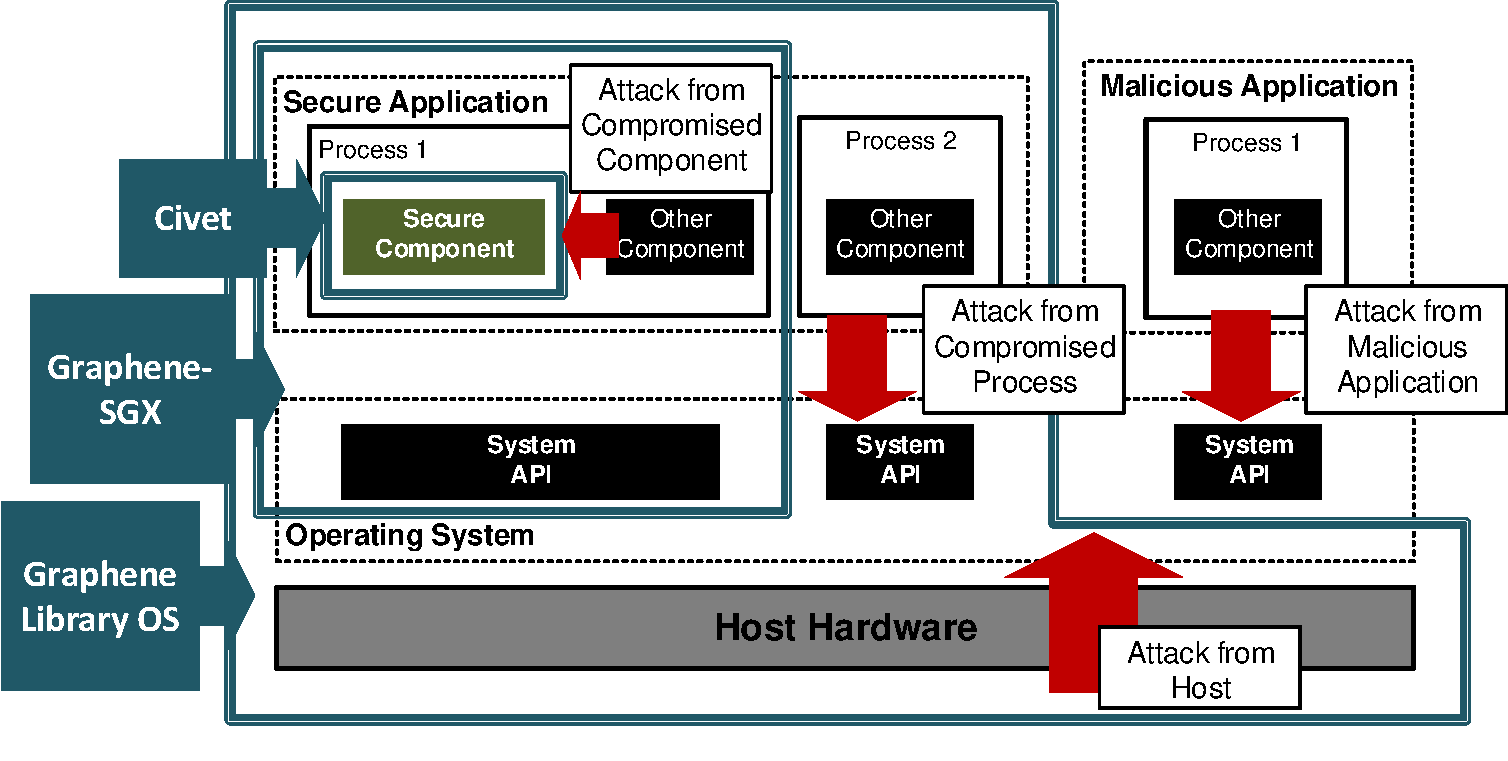
\includegraphics[width=4.5in]{figures/defense.pdf}
%\caption[Types of potential attacks on an application, and the TCB required by \graphene{}, \gsgx{} and \civet{}]
%{Type of potential attacks on the security of an application and the trusted computing base (TCB) required by \graphene{}, \gsgx{} and \civet{}.
%An application can be attacked from either the corrupted host system stack, malicious applications, or compromised components and processes in the application.
%\graphene{} can expel all untrusted applications and the system APIs that are affected by them.
%\gsgx{} further removes the host kernel and hardware, as well as untrusted processes, from the TCB. \civet{} then defends against compromised, in-process components. \graphene{} has the larger TCB, and \civet{} reduces the TCB the most.}
%\label{fig:defense}
%\end{figure}

%This thesis primarily describes three security isolation solutions,
%to defend against different levels of attack (as summarized in Figure~\ref{fig:defense}):
%\begin{compactitem}
%\item {\em \graphene{}} (\S\ref{chap:graphene}) enforces security isolation between mutually untrusting applications.
%\item {\em \gsgx{}} (\S\ref{chap:gsgx}) enforces security isolation on applications against untrusted system stacks and other applications.
%\item {\em \civet{}} (\S\ref{chap:civet}) enforces security isolation inside an application, against untrusted application partitions as well as the system stacks and other applications.
%\end{compactitem}

%\section{Security Isolation for Linux Multi-Process Applications\\ using a Library OS}
%\label{sec:intro:graphene}

As alternatives to virtualization,
\term{\liboses{}} provides a highly portable, \term{platform independent} platform,
by splitting the OS functionality from a kernel
into the application processes~\citep{porter11drawbridge,unikernels,baumann13bascule}.
%enforce isolation on mutually untrusting process,
%by essentially \emph{collapsing} OS components
%into an application library loaded into the user memory of application processes, or \term{\picoprocs{}}.
Compared with monolithic kernels,
\liboses{} minimize the reliance on the correctness or effectiveness of kernels,
to enforce isolation
on applications that distrust each other and
demand a more impenetrable barrier.
The isolation of \liboses{}
%The qualitative benefits of \liboses{},
%including isolating mutually untrusting applications,
%migrations,
%and platform independence,
is based on partitioning the OS instances
between the mutually untrusting applications,
and leaving the \liboses{} only a
narrow, restrictively defined interface to the host kernel.
%The benefits of using \liboses{} to run applications include
%isolating %the consequences of having
%security vulnerabilities in guest OSes,
%and reducing unnecessary %unneeded or redundant logics causing
%%performance bottlenecks 
%overhead for specific \picoprocs{}
%--- comparable to the benefits of using \term{virtualization},
%but at a significantly lower cost.
%%More recent \liboses{}
%%provide several qualitative benefits of virtualization,
%%such as migration and host platform compatibility.
%%Library OSes move portions of
%%OS kernel functionality into an application library.
%%In a \libos{}, the guest OS is 
%%% dp: too early for this nomenclature, I think
%% \daniela{(a libraryOS instance)},
Within a process with a \libos{}, or a \term{\picoproc{}},
the \libos{} implements the system APIs (e.g., system calls) and supporting data structures as library functions
--- mapping the system abstractions and semantics
to the narrow host interface.
%a narrow paravirtual interface to the host kernel.
Recent library OSes improve efficiency over full guest OSes by eliminating duplicated features
between the guest and host kernel,
such as the CPU scheduler, or
%eliminating guest-level multiplexing code, as the library OS supports only one application;
even compiling out unnecessary guest kernel APIs~\citep{unikernels}.
Sometimes, on top of a minimized \term{\microkernel{}} that often has the size and functionality of a hypervisor,
library OSes or applications can bypass the multiplexing of hardware resource
to improve the performance~\citep{engler95exokernel},
or separating system components
that are intensively shared and bottlenecking the applications,
such as bulk allocation of processing buffers~\citep{leslie96nemesis}.
In total, this can reduce the memory requirements of running a single, isolated application
by orders of magnitude, and similarly
increase the number of applications which can run
on a single system~\citep{porter11drawbridge,unikernels}.
In addition,
because of the narrowness of host interfaces, % is easier to implement on various platforms
%than the high-level system APIs,
the library OSes can be easily ported to an innovative, vastly distinct platform. 
A typical example is in \term{\intel{} \sgx{} enclaves},
where applications are isolated in a restricted environment that is immune to attacks from untrusted host kernel and hardware peripherals.
A \libos{} can support whole applications in enclaves,
without expanded attack surface and porting effort on the applications~\citep{baumann14haven}.
%% dp: This sentence seems a little premature
%In recent works, library OSes provide rich OS features for isolated contexts while the host OSes are untrusted

%% Library OSes reduce the memory requirements of running a self-contained,
%% isolated application process
%% %guest \daniela{I would replaced guest by "isolated process or group of processes (a libOS instance)''}
%% by orders of magnitude
%% In a cloud computing environment,
%% increasing the number of applications per server has enormous
%% economic benefits.
%% Even on a desktop or portable system, \libos{}es can reduce the overheads
%% of sandboxing untrusted code and running applications
%% designed for another OS.

%Because library OSes execute within a VM \daniela{this phrase does not read good to me because (i) it might imply the picoprocesses need hypervisor support, as misunderstood by reviewer 1 and (ii) you already emphasized the drawbacks of leveraging a VM} or lightweight process ({\em picoprocess}~\citep{xax}),
%library OSes execute with

Legacy application support is provided
in recent \liboses{}~\citep{porter11drawbridge, baumann13bascule, baumann14haven},
%, such as Drawbridge~\citep{porter11drawbridge}, Bascule~\citep{baumann13bascule} and Haven~\citep{baumann14haven},
%partial support for legacy applications is provided
by emulating the OS personalities in individual \picoprocs{}.
Among the OS abstractions and features that need to be emulated,
the emulation of
single-process abstractions,
such as accessing unshared files, or creating multiple threads in a process,
can be wrapped inside
a \picoproc{}, %, with proper level of translation and bookkeeping.
thus often relatively straightforward.
For instance, %Drawbridge loads legacy Windows applications including Microsoft Word.
Drawbridge~\citep{porter11drawbridge} provides Windows abstractions and personalities,
with 5.6 million lines of code reused from Windows 7
to emulate the complete OS personality in a single \picoproc{},
except a few features such as the Windows registry that has to be implemented
separately as in-process libraries or services.
%using in-process services. % such as the Windows registry.
However, when it comes to emulating multi-process abstractions,
%in contrast to single-process abstractions,
%multi-process abstractions 
which are commonly used by Unix applications,
%are more challenging, % to emulate in \picoprocs{},
%due to the assumption and
%narrowed interfaces of \picoprocs{}.
\picoprocs{} serving multiple processes of an application
will need to collaboratively provide shareable OS abstractions,
and more importantly, a unified OS view to the application.
%% dp: Daniela, great suggestion!  We need to make this situation seem more
%%     like the sky will fall without our help
%A key drawback of recent library OSes, however,
%is that they are limited to single-process applications.
%Yet many applications, such as network servers and
%shell scripts,
%create multiple processes
%for
%performance scalability, fault isolation, and programmer convenience.
%These applications would benefit from the efficiency and security benefits
%of a library OS.
%In order for the efficiency benefits of \liboses{} to be widely applicable,
%especially for unmodified Unix applications,
%either applications must be rewritten to implement ad hoc coordination mechanisms, or
%\liboses{} must provide commonly-used multi-process abstractions,
The multi-process abstractions to be emulated include
forking, signals, System V IPC, file descriptor sharing, exit notification, etc.
A possible alternative is
%To support multi-process abstractions, \liboses{} often have 
to rely on %sharing OS states,
the hosts' memory sharing features to share OS states.
However, memory sharing is not always an available features in the host:
for example, Drawbridge and Bascule~\citep{baumann13bascule} cannot emulate process forking because copy-on-write memory sharing is not a platform-independent features.
Furthermore, when Haven isolates applications
in enclaves,
memory sharing is strictly forbidden by the hardware platform,
to prevent leaking secret to other enclaves.
In a word, emulating OS abstractions and personalities can fundamentally
oppose the assumptions or limitations of the system,
causing obstacles to supporting legacy applications.


%\begin{figure}[t!]
%\centering
%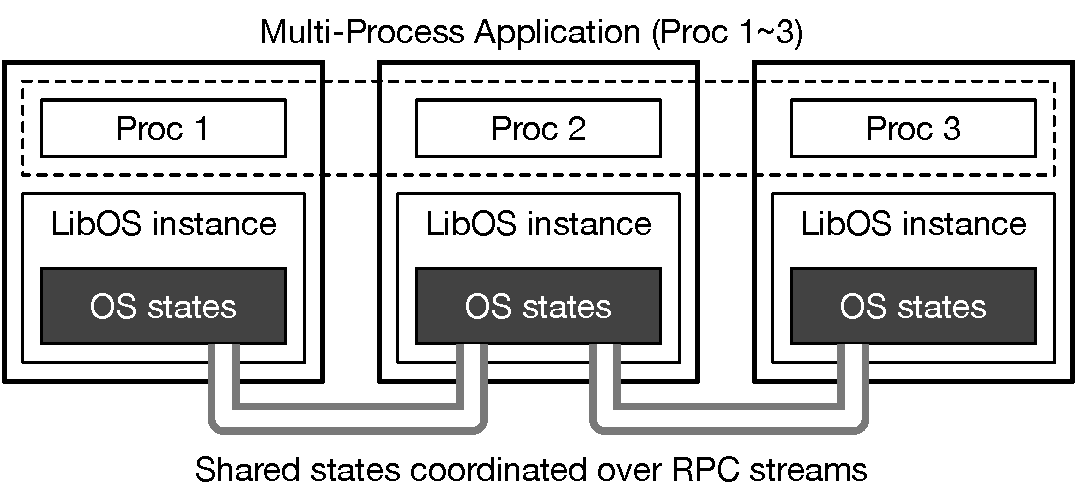
\includegraphics[width=0.75\linewidth]{graphene/figures/concept.pdf}
%\caption[Multi-process abstraction model of \sysname{} \libos{}]
%{Multi-process abstraction model of \sysname{} \libos{}. For each process of an application, a libOS instance will serve system calls and keep local OS states. States of multi-process abstractions are shared by coordinating over host-provided RPC streams, creating an illusion of running in single OS for the application.}
%%\vspace{-.1in}
%\label{fig:graphene:concept}
%\end{figure}

%We present {\em \graphene{}}, a Linux-compatible \libos{} to secure unmodified, Linux multi-process applications.
%In \graphene{}, multiple \libos{} instances collaboratively implement
%multi-process abstractions,
%yet appear to the application
%as a single, shared OS.
%\graphene{} instances coordinate state using remote procedure calls (RPCs) over
%host-provided, pipe-like streams.
%In a distributed POSIX implementation, placement of shared state and messaging complexity
%are first-order performance concerns.
%%We chose to shift implementation complexity into the library OS
%%in order to uphold simple enforcement of security isolation in the host.
%By coordinating shared states across \libos{} \picoprocs{,
%\graphene{} is able to create an illusion 
%of running in a single OS
%for multiple processes in an application.

%Previous library OS designs ensured security isolation of independent applications,
%comparable to a VM, by keeping a relatively narrow host ABI.
%We selected the \sysname{}
%design because it strikes a unique balance between
%and robust, flexible security enforcement.

%The design of \graphene{} ensures security isolation of
%mutually untrusting, multi-process
%applications on the same host.
%Essential to this goal is
%minimally expanding the host ABI to support multi-processing,
%as well as leveraging RPCs as a natural point to mediate inter-\libos{} communication.
%RPC coordination among \graphene{} instances can be dynamically disconnected, facilitating novel sandboxing
%techniques.  For instance, we develop an Apache web server extension that, upon logging in a given user,
%places the worker process's \libos{} in a sandbox with access to only that user's data.
%We expect more nuanced degrees of trust are possible in future work.

%\graphene{}'s design gives the user and system administrator a high degree of flexibility
%in isolating arbitrary groups of unmodified application processes,
%while upholding the efficiency and host compatibility benefits of recent \liboses{}.


The key to emulating multi-process abstractions in a \libos{},
especially when memory sharing is not safe or available,
is to coordinate shared OS states
across \picoprocs{} using limited host abstractions.
%The \libos{} of related \picoprocs{} %that accompany application processes
%must collaboratively provide a unified OS view
%to the application.
The OS states needed to be coordinated
are primarily in three types:
process states that are inherited at process creation
(e.g., {\tt fork}, {\tt execve});
abstraction states that are shared among related processes
(e.g., signals, \sysvipc{} semaphores);
and namespace states to locate the owners of abstractions
(e.g., process IDs, \sysvipc{} keys).
A \libos{} that implements all the idiosyncratic OS states
must not overly expand the host interface,
and compromise the security isolation or platform independence of the system.
%and thus increase the risk of
%allowing malicious applications to compromise the host kernel.
As a solution, we present \term{\graphene{}},
a Linux-compatible \libos{} that collaboratively implement
various Linux multi-process abstractions,
yet appear to the application as a single, shared OS.
\graphene{} instances coordinate all OS states using remote procedure calls (RPCs) over
host-provided, pipe-like streams.
The use of host RPC streams
does not expand the host interface already used by a single \picoproc{},
and can be naturally isolated
by sandboxing the RPC streams from the host.
%with the application.
%In a distributed POSIX implementation, placement of shared state and messaging complexity
%are first-order performance concerns.
%%We chose to shift implementation complexity into the library OS
%%in order to uphold simple enforcement of security isolation in the host.


%\fixmedp{After a complete draft is written, coalesce all goals and make sure they are addressed early on.  We are doing some scatter-shot motivation}

%\section{Isolating Native Applications on Untrusted Hosts}
%\label{sec:intro:gsgx}

%The complexity of modern operating systems has become
%a major source of security vulnerabilities,
%pressuring developers to seek solutions to exclude the host OSes
%from their trust models.
%The untrustworthiness of OSes get severe when applications are run in the cloud,
%because the applications may cohabit with compromised tenants,
%or be hosted by malicious providers.

%Existing works provide isolated execution of applications
%on untrusted operating systems or host hardware,
%using either hypervisors~\citep{criswell2014virtualghost, flicker, inktag, zhang2012mushi} or security hardware~\citep{intelsgx, secureblue++}.
%Especially security hardware such as \intel{} \sgx{}~\citep{intelsgx} can defense against hardware-level attacks,
%with low execution overhead.
%\sgx{} is a set of new instructions introduced in the latest \intel{} CPUs,
%to create a encrypted memory region called {\it enclave}
%in the application's address space.
%\sgx{} guarantees that only signed code loaded in the enclave can access the sensitive data stored in the enclave memory.

%Protecting applications without the requirement of trusting the hosts
%has become valuable in modern computer systems for many reasons.
%The complexity of the existing commodity operating systems has become a major source of
%vulnerabilities to exploit.
%Once the host operating systems are compromised,
%any security mechanisms enforced in the applications can be easily circumvented.
%If the applications run in the cloud,
%the hosts have to be controlled by the cloud providers,
%which is capable of compromising both host operating systems and hardwares.
%The attacks from the cloud is possible even if
%the operating systems' vulnerabilities are never exploited.

%However, isolating an application with \sgx{} enclaves
%requires additional porting effort,
%to partition the application into a signed, trusted binary,
%and the rest.
%Only the trusted binary will be loaded in enclaves.
%The enclave will interact with the rest of the application
%through an {\em untrusted interface},
%to pass input and output of the isolated execution,
%and access OS features such as files and network.
%For a complex application such as a network server or a desktop GUI,
%the effort to partition the application is too high,
%and the untrusted interface is often too large,
%given the complexity of interaction between the enclave and the rest of the application.

%Unfortunately, leveraging SGX for security
%often requires rewriting the applications to a large extent.
%Because the OSes cannot be trusted,
%enclaves are not allowed to directly access any system interface
%for any OS features
%such as files, networks or scheduling.
%Only a limited subset of system library API can be exported in enclaves;
%for example, the software development kit for SGX
%only supports spin-locking as scheduling tool,
%because other primitives require cooperation from the OS.


%With the support of a \libos{}, developers can port an application to \sgx{} with minimal effort,
%using a {\em non-partitioned model}~\citep{baumann14haven}.
%The non-partitioned model loads the whole application binary into the enclave,
%and a \libos{} to support the OS features.
%The benefits of using a non-partitioned model also include
%limiting the untrusted interface to a narrow, fixed interface,
%and the fact that the application is protected ``as is''
%--- especially useful for privacy-preserving applications.


In particular, the platform independence of \liboses{}
allows porting legacy applications to platforms with more restricted interfaces
and functionalities than monolithic kernels,
such as \intel{} \sgx{} enclaves.
The essence of isolating applications using \liboses{} in enclaves
is to ensure
the security benefits promised by the platform,
%in an system enforcing stronger security isolation
%on legacy applications,
%such as Haven~\citep{baumann14haven},
%it is necessary
%%the system must not only emulate the personalities,
%to provide the security benefits promised by the platform
%(i.e., enclaves).
%%instead of simply emulating the personalities.
%For instance,
%the security benefits of enclaves
including application integrity,
sealing confidential information,
and attestation.
%These benefits must be also provided by systems that use enclaves to isolate legacy applications.
An existing system, Haven~\citep{baumann14haven},
packs a Windows-compatible \picoproc{}
into an enclave,
using an encrypted virtual disk
securely provisioned from a remote, attested server.
Haven essentially provides a trusted path to safely load application and \libos{} binaries,
as well as mediating all input and output to the host.
%as the trusted path to safely load application and \libos{} binaries.
%Haven relies on
%%the \libos{} to
%securely provisioning an encrypted virtual disk
%from a trusted, remote server,
%to ensure a \emph{trusted path} to
%load authenticated application binaries
%and redirecting IOs,
%yet appears
%completely transparent to the application.
The only limitations in the model of Haven, however, 
%are the huge TCB (trusted computing base)
%caused by the \libos{} (209MB in total),
are the lack of multi-process support,
and being overly reliant on the remote server.
% and being incapable of isolating multi-process applications.
% especially in the finer, per-process granularity.
Addressing these issues,
by porting \graphene{} to enclaves
(\term{\graphenesgx{}}),
we reassure multi-process, UNIX applications in a multi-enclave environment.
The application integrity in \graphenesgx{} 
is validated on unencrypted,
regularly distributed binaries,
using checksums
signed by the hardware-attested measurement
--- an off-line model without relying on
remote servers.
\graphenesgx{} ensures that
process creation in enclaves can be scalable, and individually configured
--- a parent enclave can identify and restrict
the application binaries to be loaded into any child enclaves it creates.
%to isolate multi-process applications in a multi-enclave environment.
%The coordination of \graphene{} based on RPC streams
%allows isolated \picoprocs{} to build a trusted path for OS coordination,
%by attesting and encrypting the RPC streams.
%\graphene{} verifies binary integrity using per-binary checksums,
%to rid most application behaviors
%of the dependency on remote trusted servers,
%and to allow each \picoprocs{} be attested and provisioned individually.



%To alleviate the pain of migrating applications to SGX,
%recent works like Haven~\citep{baumann14haven} provides a mechanism
%of loading native applications into enclaves,
%alongside a library OS to facilitate rich OS features.
%These systems are called ``shielding %systems''~\citep{xu15controlledchannel},
%which means these systems can secure execution environments
%without trusting the host.

%A primary drawback of the non-partitioned model is the huge TCB loaded into the enclave.
%In the partitioned model, only minimal code needed for the isolated execution will be loaded into the enclave.
%However, in the non-partitioned model, the whole application must be loaded into the enclave,
%in addition to the TCB contributed by the \libos{}.
%For instance, size of the \libos{} used in \cite{baumann14haven} is 209MB,
%which yields significant expansion to the original TCB.
%
%We present {\em \gsgx{}}, a port of \graphene{} \libos{} on \sgx{}, to secure unmodified Linux applications in \sgx{} enclaves{}.
%The support for Linux applications
%has been missing in the non-partitioned model,
%which is a missed opportunity according to the 75\% market share of Linux cloud providers~\citep{linuxcloud2014}.
%\gsgx{} supports most OS features provided by \graphene{}
%including both single- and multi-process abstractions.
%
%The design of \gsgx{} ensures the minimal enclave TCB
%that can be achieved without further partitioning any application binaries.
%The integrity of the loaded application binaries
%is enforced in a fine-grained fashion:
%each binary must be signed and checked individually,
%and only binaries that are actually needed will be ever loaded.
%For multi-process applications,
%\gsgx{} isolates each \picoproc{} in a separate enclave,
%thus every \picoproc{} can execute and be attested separately.
%In a nutshell, \gsgx{} tries to honor and exploit the established partitioning in multi-process applications,
%with the benefit of minimizing the porting effort from using the non-partitioned model.


\paragraph{Improving Efficiency with Legacy Support.}
One of the other first-order requirements in systems, besides legacy support,
is to pursue low latency or high throughput,
according to how users define quality of service.
Nevertheless, there is a trade-off between the emulation of OS personality
and the efficiency of system operations.
\graphene{}, for instance, coordinates OS states %for multi-process abstractions
over PRC streams,
and requires strategies to mitigate the significant RPC coordination overhead.
%will cause nonnegligible overhead to the latency of IPC,
%in comparison with coordination by memory sharing. % in the kernel or in the \picoprocs{}.
%However, when designing a \libos{},
We observe, in a distributed UNIX implementation,
placement of shared OS states and
messaging complexity
are essentially the top performance factors.
%%there are opportunities to identify and remove unneeded or redundant
%%overhead or bottleneck,
%%especially on the critical or common paths.
%%%frequent operations.
%%An example of reducing overhead
%%is to remove redundant permission checks in \liboses{},
%%because \picoprocs{} rely on the host kernel to enforce security policies.
%%Similarly, to compensate the overhead of IPC
%%in a distributed implementation, placement of shared OS states and messaging complexity
%%will be the first-order performance concerns.
%For \picoprocs{} that most frequently access an abstraction state,
%place the state in this very \picoproc{}
%will optimally avoid the need for coordination over RPC streams.
Improving the coordination overhead will require placing the OS states in the most frequency accessing \picoprocs{},
and reducing round trips of RPC messages.

\paragraph{Partitioning Legacy Applications.}
Beside supporting whole applications,
%and derive principles to improve the result of implementation.
we also explore the opportunity of partitioning a legacy application,
in a model where it is split into
trusted and untrusted components that are isolated by platforms like enclaves.
The partitioned model for porting to enclaves
is commonly used for quarantining the extremely sensitive execution
in an application.
The purpose of partitioning is to
defend against the whole, untrusted host systems (except the CPUs)
as well as other less sensitive components,
in order to minimize the trusted computing base.
The weakness of the model is,
partitioning an application requires additional effort to identify and separate
the execution that needs to be protected,
and the effort becomes unacceptably expensive when the application is considerably sophisticated.
In particular, we are targeting applications implemented
in a managed language such as \java{},
which are more likely to be automatically compartmentalized
using programming language techniques.


%We observe that in order to partition a system or application
%in finer granularity,
%%such as an extremely sensitive component,
%%legacy code reuse will become even more challenging.
%%In this case,
%%inevitably,
%applying techniques from programming languages %and code analysis
%will become necessary.
%Specifically, one technique that developers will need is automated compartmentalization of legacy code.
%%The reason is, 
%Unless the partitioned component code is compact and simple,
%the effort required
%for cleanly and minimally partitioning the code
%will be too high.
%For an application developed in a managed or object-oriented language (e.g., \java{}),
%code compartmentalization can be effective enough to create close-to-optimal partitioning.

The motivation for pursuing \java{} application partitioning
is two-folded.
On one hand,
many enterprise or cross-platform applications
are developed in \java{},
but so far no enclave support for whole or partial \java{} applications
is ever provided.
%To load an application into an enclave,
%both the execution and interface of the application code
%have to be static
%ever since the enclave starts.
%Because \java{} classes are dynamically loaded and managed by \java{} VMs,
%extra support from the system will be necessary.
On the other hand,
execution isolated in an enclave must be unconditionally trusted;
if any vulnerabilities exist in the execution,
the attack can infiltrate from the untrusted host to compromise the isolation.
However,
just as the whole application,
the isolated part is also hard to completely eliminate vulnerabilities.
%an application or component isolated in an enclave must be %verified to
%immune to security vulnerabilities,
%otherwise there will be risks of leaking the enclave secrets.
By allowing developers to port \java{} applications into enclaves,
protection mechanisms based on
the characteristics of \java{} language,
such as type checking, information flow tracking among objects,
can further ensure the soundness of isolated execution.
The automated partitioning of \java{} applications into enclaves
is an ongoing work.


%
%Haven effectively migrates native Windows applications to enclaves,
%providing a shortcut for developers
%to easily boost the security of their products.
%However, there are several limitations in Haven, including
%excessive trusted computing base (TCB),
%a restrictive model of adapting applications,
%and missing support for Linux or multi-process applications.

%We present \gsgx{}, a \libos{}-based shielding system
%targeting Linux multi-process applications,
%as improvement to the Haven model of migrating native application to SGX.
%\gsgx{} is derived of \graphene{}~\citep{tsai14graphene},
%which supports 139 out of 300 Linux system calls.
%\graphene{} runs numbers of popular applications
%such as Apache web server, OpenJDK virtual machine, or shell scripts,
%all of which relies on multi-process abstractions
%such as {\tt fork}, {\tt execve}, signals or System V IPC.




\paragraph{Measurements for System Completeness.}
In general, due to the complexity of implementation or preserving
the complete specifications,
developers must prioritize the development based on
what they believe to be more important
--- what will impact or satisfy more applications or more users.
Especially for innovative systems like \liboses{},
developers struggle to evaluate the progress in a partial prototype.
%From improving legacy code compatibility in different systems
%(Linux to \graphene{}),
%we observe that system developers including us
%routinely make design choices based on 
%what they believe to be the common and uncommon behaviors of a system.
%For instance, in \graphene{}, we start with handpicking the abstractions and specifications
%that we believe to be more important to the applications.
%When optimizing Linux file system directory cache,
%we shorten the latency of {\tt stat} and {\tt open} system calls
%at the expense of {\tt rename} and {\tt chmod},
%assuming that {\tt stat} and {\tt open} are the more commonly used operations in majority of applications.
%%In the case of a general-purpose OS, determining
%%exactly what the common case is can be challenging.
%In general,
%a developer's view of what system APIs are important is skewed towards
%the developer's preferred workloads.
%%the choice of what features matter skews heavily towards
%%workloads particular developers use.
%Similarly, developers who struggle to evaluate the impact of a 
%change on compatibility
%must implement every abstractions and specifications,
%and then be able to reason about the completeness of legacy support.
%support of legacy application in the product system.
At the center of these problems is the missing of information about how system abstractions or APIs are used in the run-time.
%and a metric to estimate the completeness of legacy applications that can be supported
%for any random users.
In search of better methods for
evaluating the legacy support,
we conduct a study of Linux system APIs usage among a large sample of Debian/Ubuntu x86\_64 applications,
weighted by the application popularity
collected by the Popularity Contests~\citep{debian-popularity, ubuntu-popularity}.
Based on the study,
we create a measurement
for estimating the fraction of applications installed by a user
that can plausibly use the system.
For instance, the current \graphene{} prototype,
in which we hand-pick Linux system calls according to the applications for experiment,
can support the complete API footprint
in 0.42\% of applications installed by a user.
The data-driven, principled strategy shows than \graphene{} can be improved to
supporting 21.1\% of applications,
by simply adding two missing system calls, {\tt sched\_setcheduler} and {\tt sched\_setparam}.

%We create sensible, representative metrics,
%which measure the effects of both applications and users.
%Using the metrics and insights from the study,
%the significant improvement on legacy application support in \graphene{} is demonstrated
%if we guide the development using this approach.

%Summarizing all contributions of the thesis,
%we explore the solutions and principles,
%to implement OS support for legacy applications in either 
%isolated systems
%(i.e., \graphene{} \libos{}, enclaves) 
%or optimized legacy OS components
%(i.e., Linux file system directory cache).






%By supporting Linux multi-process applications,
%\gsgx{} simply applies to a broader range of cloud-based applications
%than Haven.
%Survey shows that Linux yields a market share of up to 75 percent in
%enterprise cloud providers~\citep{linuxcloud2014}.
%This data suggests majority of the existing cloud users can
%more easily adopt \gsgx{} than Haven.

%\gsgx{} uses a different model from Haven
%to bootstrap the trust of loaded applications.
%Haven builds up the trust by packing all binaries
%in an encrypted virtual disk,
%with secret key provisioned consensually from a remote server
%trusted by the clients.
%Contrastingly, \gsgx{} relies on a model directly derived from
%the trust model of \sgx{},
%by including applications' checksums
%into the enclave measurement to be attested by hardware.
%\gsgx{} can migration applications for enclaves off-line,
%and share binaries (e.g., shared libraries) to save bandwidths for deployment.
%
%Security-wise speaking,
%\gsgx{} provides a way to reduce the TCB of enclaves,
%with a smaller code footprint
%and applications natively partitioned as processes.
%Haven in general yields a large TCB
%including a \libos{} as large as 209MB,
%and application binaries around 10s \textasciitilde 100s of MB.
%The image of \gsgx{} is merely 10MB,
%and Linux applications generally follow the principle of dividing
%code into smaller, more testable binaries.
%\gsgx{} isolates multiple binaries (or processes) of an application
%in separate enclaves, and authenticates inter-process coordination
%by binary-based policies.
%Even if an enclave is compromised, other enclaves of the same application
%can still stay secure as long as
%critical information never flows to the victim.
%
%\gsgx{} provides cloud users
%ease of shielding Linux applications
%and flexibility of implementing any desired security model
%suitable for each binary.

%\section{Combining Isolated Execution with Language Protection\\ for Partitioned Applications}
%\label{sec:intro:civet}

%% \fixme{Chia-Che Tsai's opening}
%% Modern security hardwares such as TPM or \sgx{}
%% provide hardware enforced guarantees of security properties
%% even upon %untrustworthy hosts with
%% compromised operating systems or tampered hardwares.
%% The reasoning of security using these hardwares
%% is often founded as follows:
%% An untamperable hardware package such as CPU will guarantee
%% the integrity of applications loaded
%% exactly identical to the images signed by clients.
%% However, to achieve overall security,
%% the clients are still responsible for ensuring that no vulnerabilities
%% within the signed images
%% will compromise the security properties in runtime.

%%\fixmedp{I would start by motivating the goal of application partitioning.
%%I think you could add a little more here, but this is a rough sketch.}
%For applications that handle sensitive data such as private keys,
%or implement proprietary algorithms,
%running on a untrusted host whose hardware and hypervisor
%may be compromised is a huge risk.
%%, such as medical applications, or 
%%implement proprietary algorithms, such as algorithmic stock trading.  
%%These applications are composed of 
%%libraries and other code from third parties, and may run on 
%%hardware and hypervisors provided by an untrusted cloud provider.
%%Using the partitioned model the developers can 
%%bound the effort to protect sensitive data and algorithms,
%%while still taking advantage of inexpensive code and cloud hardware.
%%A partitioned application isolates sensitive data and code, typically using
%%language or hardware techniques.
%If users run these applications in isolated execution such as \sgx{},
%due to the complexity of the applications,
%the cost of partitioning and porting the applications may be too high to pay.
%However, as discussed in \S\ref{sec:intro:gsgx},
%using the non-partitioned model, the application must tolerate a much larger TCB in the isolated execution,
%whereas a large fraction of the TCB is less sensitive.
%
%A solution to this dilemma
%is to automate the partitioning using language techniques.
%For instance, applications implemented in managed languages like \java{}
%are easier to partition,
%if a few hints about the sensitive data can be provided by the developers.
%Since \java{} classes are often well modularized,
%an automated language-level tool can analyze the minimal supporting classes to process the sensitive data,
%creating a clean partition with more reasonable TCB.

%%Why SGX
%%\fixme{Bhushan's opening}
%At the hardware level, 
%new CPUs are offering features to protect application-level code and data
%from a  compromised or malicious system software stack,
%including the OS or hypervisor, or simply isolating portions of the 
%application address space from the rest of the application.
%Examples include SX~\citep{sgx-manual}, 
%%\fixmedp{Can we mention/cite others? IBM and ARM?}
%IBM SecureBlue++~\citep{secureblue++}, and ARM TrustZone~\citep{trustzone}.
%%are offering models of mutual distrust, which facilitate protecting
%%an application from a
%SGX offers %One feature of SGX is restricted
%entry points to an encrypted region of memory, called an {\em enclave}.
%Encryption and remote attestation 
%prevent the hypervisor or OS from reading or modifying the enclave's contents,
%and validate that the enclave was correctly initialized.
%This in turn
%can exclude 
%a cloud provider's hypervisor or OS from the application's trusted computing base (TCB),
%requiring only trust in the hardware manufacturer (i.e., Intel).
%%Remote attestation can also validate that an enclave was correctly initialized.
%%Enclaves also provide remote attestation, where a client
%%can ascertain whether the hardware is genuine Intel, and that the application was
%%loaded correctly.
%SGX also offers protection against malicious devices off the CPU package,
%such as a compromised storage device.


%Besides automated partitioning,
%securing \java{} applications in \sgx{} opens opportunities to hardening the security of isolated execution,
%using language-level protections
%~\citep{bittau2008wedge,brumley2004privtrans,khatiwala2006data}.
%For instance, the type-checking feature in the \java{} language
%can avoid the risk of exploitable pointers or control flow errors,
%which is significant in an unsafe language like C
%~\citep{nergal2001libc,bletsch2011jump,checkoway2010return}.
%
%In addition, although SGX can restrict enclave entry 
%to a few predefined entry points,
%the developers still have to reason about what the soundness of the
%entry-point definitions, protection against malicious inputs,
%and the code paths that must not inadvertently leak sensitive data.
%For instance, Iago attacks~\citep{checkoway13iago}, where an OS offers malicious system call return values,
%can be notoriously difficult to defend against from an enclave;
%although limited countermeasures exist for the OS API (typically with the cooperation of a 
%trusted hypervisor)~\citep{kwon2016sego},%\fixmedp{cite the asplos 16 inktag paper},
%there are no off-the-shelf defenses against Iago-style attacks from the compromised application code.

%Further, SGX is designed to run a small, native code library inside of a larger
%application; support for running managed languages in an enclave is currently limited.  
%Writing a security-sensitive application in an unsafe
%language like C dramatically increases the risk of exploitable pointer or control flow errors, which ultimately disclose sensitive data or undermine the integrity of the enclave.

%Modern security hardware
%such as  provides hardware protection to applications
%especially the ones deployed in the cloud,
%so that the applications do not have to trust the privileged
%OS layer controlled by the cloud provider. 
%against malicious system stacks, including OS, hypervisors or devices. 
%In principle, these hardware techniques 
%Hardware protection between applications and their hosts is appealing
%in cloud computing, because the cloud client 
%need only trust the 
%the cloud provider's hypervisor can, in principle, 
%be excluded from the application's trusted computing base (TCB).
%These hardware protection is especially essential for cloud computing, due to the multi-tenant environment and potentially compromisable providers.
%\fixme{I want to emphasize it can defend against hardware attack.}
%This type of hardware creates a sanctuary for the most security-sensitive
%components of an application---

%For instance, SGX creates a encrypted memory region 
%called {\em enclave} within the memory space of an application,
%which can only be accessed by verified code from the users.
%\fixme{I rather not emphasize partitioning so early, it's not the only way of using enclave.}
%SGX lets the developer partition the application into two parts --- 
%security sensitive and non-security sensitive parts. The security
%sensitive part of the application is run in an hardware isolated
%sandbox called enclave, while the non-security sensitive part runs
%normally outside the enclave.
%% SGX guarantees not only the integrity of loaded application image,
%% but also the confidentiality
%% of application data, %in enclave,
%% avoiding any information leakage to the untrusted exterior world.
%SGX provides a fail-safe way to prevent information leakage from the enclave:
%by guaranteeing the integrity of a measured %and verified
%application binary
%and the confidentiality of application data in memory.
%the OS or hypervisor are simply stopped from peeking any application data, unless the isolated applications release any information. 

%Language-level techniques can offer more sophisticated insights into how
%to partition the application, as well as stronger protections ~\citep{bittau2008wedge,brumley2004privtrans,khatiwala2006data}.
%%\fixmedp{Can we bless some language-level app partitioning tools here?}
%Similarly, managed languages such as Java, with type-checking,
%can prevent memory corruption attacks,
%while applications developed in C or C++ are often prone to memory-bug exploitation.  
%Because Java is memory safe, it is immune to known control flow attacks, such as return-oriented programming,
%where control flow is manipulated by unsafe writes to return pointers on the stack or function pointers in objects.

%protection prevents applications from being compromised by
%vulnerabilities that exist inside the applications.
%The vulnerabilities include mistakes made by developers, such as semantic and configuration bugs,
%and unbound application behaviors that can be exploited by attackers,
%such as memory attacks or control flow attacks.
%Based on the different languages used by developers,
%applications can be offered stronger language specific security guarantees.

%Although combining isolated execution and language protections
%is beneficial for partitioned applications,
%the synthesization of the two mechanism can be difficult in practice.
%%In general, hardware protection and language-level protection 
%%provide separate security guarantees.
%%Unfortunately, developers often struggle to combine both types of protection, due to the limitations and lack of support for both approaches.
%We focus on the combination of \sgx{} and \java{} as a running example:
%\sgx{} are designed to run native code that is primarily developed in C or C++.
%Without further support, a partitioned \java{} application
%cannot be directly loaded into an enclave.
%There is also no API support for \sgx{} features in \java{},
%making it challenging for \java{} applications to use any \sgx{} features to their advantage.
%%Developers often have to create an ad hoc integration of hardware and language-level protection,
%%or they are forced to exclusively expose the application between
%%attacks from the system stacks and vulnerabilities inside the applications.
%The current state-of-the-art of secure more complex applications with \sgx{} is to develop ad hoc solutions that target specific use cases.
%% approaches of combining
%%language and hardware protection often rely on ad-hoc solutions that
%%are specific to certain use cases or technologies.
%For example, \cite{vc3} use \sgx{} to secure data analysis in a MapReduce framework supporting C++
%--- instead of the Hadoop framework that generally supports \java{}.

%% dp: this sentence seems off track, unless you want to say something about ``this has to be in C''
%Similarly, S-NFV uses SGX to isolate states of Network Function Virtualization Applications~\citep{shih2016s}.

%\fixmedp{Please check the previous 2 sentences for accuracy; if I'm wrong, try to say something more crisp.
%Also, any other important related work here?}
%to utilize SGX hardware in language runtimes,
%a set of APIs may be exported through the native interface to support certain high-demand use cases, such as Hadoop workloads
%Although these existing solutions nicely support a part of the users,
%and potentially have demonstrated some common wisdom for combining the language and hardware protection,
%the problem of how to generalize the approach
%to cover more use cases or technologies that the authors haven't forseen,
%still remains unsolved.

%% dp: This paragraph is a little too much philosophy for me.  Cutting for now, but can bring some fo this back later in the intro if needed.  I think it would be better for explaining the benfits of Civet.
\begin{comment}
We use SGX vs Java-based protection as an example,
to show how the guarantees ({\em what is secured?})
and features ({\em how is it secured?}) of hardware protection
can be properly modeled at the language level,
so that language protection mechanisms can be extended
to mitigate vulnerabilities in hardware protection. 
For instance,
SGX hardware provides isolation between multiple
levels of security sensitivity in an application process,
by building another privilege level that bypasses the OS or hypervisor.
We model this hardware guarantee at language level by asking the developers
to identify the multi-level security sensitivity in the application.
The developers do not have to worry about
when to enter or leave the enclaves,
what information to flow out of the enclaves,
or even how SGX enclaves fundamentally work.
The language features
such as implicit and explicit information flow tracking can be {\em leveraged}
by the low-level component that interfaces with SGX enclaves
as the criterion for whether certain information
is safe to be released from the enclave.
\end{comment}
%while 
%


%to the privileged
%or un-privileged code outside the \enclave{}.

%One of the primary concerns on the security of enclaves is
%the strong assumption
%that enclaves' security guarantees rely on---
%The security guarantees of hardwares like SGX rely on a strong assumption:
%To provide the confidentiality guarantees,
%the code running in an enclave must not
%the secured environment (\enclave{}) must not
%have %any bugs or
%vulnerabilities that can be exploited for causing any information leakage.
%However, without language support, it is hard to ensure that
%the enclave code is
%free of vulnerabilities, especially if written in C---which provide no memory safety.
%the SGX only supports programs 
%written in C or C++, and it is extremely difficult to find
%all the memory corruption bugs in the enclave code written in C or C++.
%Without memory safety, 
%the control flow of the code %within the enclave
%can be manipulated by exploiting memory corruption.
%This type of vulnerabilities will lead to information leakage,
%defeating the purpose of using SGX enclaves.
%secure hardware such as
%SGX in the first place. 


%% Lack of memory safety using C or C++ in SGX-secured environments \fixme{maybe spell out why it's hard for SGX}
%% enervates any software approaches to reinforce application security, including control flow and information flow integrity, 
%% %These memory corruption bugs can be exploited to change the control flow within the \enclave{} 
%% %as well as leak confidential information outside the \enclave{},
%% defeating the purpose of using %SGX
%% secure hardware in the first place. 
%% \fixme{perhaps justify why not use verification?}

%One solution to guarantee memory safety in applications is to use 
%Using a managed language such as Java
%to implement the security sensitive code
%is a solution to guarantee
%can provide the memory safety
%required by an enclave.
%The solution to avoid the memory corruption bugs is to use a memory safe managed
%language like Java. Thus, partitioning an application written in language such as 
%Java and running the Java based security-sensitive code in an \enclave{}
%can help provide the control flow as well as information flow guarantees that SGX is
%designed for.
%Moreover, Java is widely used to develop many enterprise applications,
%that can improve their security guarantees by leveraging the SGX feature.
%However,
%in absence of Java language support for SGX enclave, 
%it is cumbersome to leverage security guarantees of SGX directly,
%unless developers 
%rewrite the security-sensitive components in C or C++, 
%and integrate %this new code with the original application using a 
%using a foreign function interface such as Java Native Interface (JNI).
%Java Native Interface (JNI).
%to integrate with the rest of the enterprise application.
%Moreover,
%Reimplementing the security-sensitive components
%of the application 
%in C or C++
%Rewriting in C or C++ 
%essentially voids any security benefits brought by managed languages.
%the memory safety guarantees provided by Java. 

%Additionally, having runtime support for SGX in %a managed language like
%Java
%has many benefits.
%Code written in Java %a managed language
%is easier to 
%modularize, partition and reason about the security and information flow.
%Thus, providing Java runtime support for SGX can help provide stronger security guarantees
%for applications running in an \enclave{} as well as make numerous applications
%written in Java secure against shared vulnerabilities of the privileged layer.
%Also, imported library classes can be also secured when used in applications instead of be blindly trusted.
%\fixmebj{Find one more benefit of using Java.} 
%Moreover,
%Java is widely used to develop many enterprise applications,
%which can benefit from the security guarantees of SGX
%without the cost of reimplementation.
%that can improve their security guarantees by leveraging the SGX feature.

%Another notable impediment for effectively leveraging SGX 
%feature in a managed language
%is the trouble developers
%have to endure to partition an existing application into two clear parts and design the interface
%between these two parts. There is a very good chance that an unsuspecting developer may copy
%information which is either security sensitive or derived from security sensitive data to outside 
%the enclave,
%undermining the hardware security guarantees provided by SGX. Thus, we need an 
%easy to use language runtime support for SGX
%that can shield the developer from the complexity of determining whether security sensitive information 
%is leaked outside the enclave.


%\fixme{Bhushan, read until here.}
%a framework that help Java developers partition their code
%between security sensitive and non-security sensitive parts by adding a few lines of annotations.
%The framework automatically partitions the code into two separate binaries which are run 
%inside and outside the enclave such that the least amount of code as indicated by the
%developer annotations is run inside the enclave, and transparently creates 
%the necessary interface between the two parts. 
%% The interaction between the 2 parts of the application
%% is handled using \emph{reflection library}.
%% We perform dynamic information flow tracking 
%% and control the information flow at the endpoints of the \enclave{}.
%% By default, the framework automatically encrypts any object leaving the \enclave{}, but the
%% developer can override an endorser method to explicitly let some objects pass in the clear --- e.g.,
%% a ciphertext object. Based on information flow tracking, if an endorsed object is affected by some other
%% security sensitive data before leaving the enclave, the developer has to endorse it again.
%We use dynamic information flow tracking to enforce the policy that no information that is security sensitive or
%derived from other security sensitive information is flowing out of enclave in clear, without explicit
%developer directive.
%% Our framework provides ease of partition as well as makes it explicitly clear to the
%% developer when some information is flowing out of enclave in clear. 
%This ease of use and explicitness helps
%developer reason about the security of the code more clearly.
%Civet achieves three properties: {\em security}, {\em practicality} and {\em usability}.
%Civet is designed to protect the confidentiality and integrity of 
%real-world application code. 
%Civet not only requires very little developer effort to adopt, but also provides the developer
%with essential insights into how data can flow through the application,
%leading to better reasoning about the isolation properties of the partition.
%low developer effort,
%requires minimal porting effort,
%and provides ease of reasoning about the security strength.

%\fixmedp{I would refocus a bit on the contributions.  Make sure I don't overstate}
%Civet addresses design challenges at both the hardware and language level.
%%one from each of hardware protection and language-level protection.
%To extend hardware protection, Civet contributes techniques for dynamically loading JAVA classes in enclaves
%with the same code integrity verification as native, static binaries.
%Civet uses the \graphene{} library OS~\citep{tsai14graphene} to facilitate 
%running a restricted JVM runtime in an enclave.
%to facilitate and restrict the interface size of a 
%and prove the measurement of loaded classes as part of the hardware-generated attestation.
%Then Civet verifies and attests loaded JAVA classes on the basis of measurement checking and attestation generation from the hardware.
%On the other hand, Civet has to adopt language-level protection to enforce information flow policies against leakage over the border of enclave.
%Civet enforces information flow policies at the border of the enclave by incorporating
%Phosphor~\citep{bell2014phosphor} instrumentation on all classes in the enclave,
%tracing both explicit and implicit flows from any confidential data,
%and preventing tainted information from leaving the enclave by any interface, 
%except via explicit declassification by the developer.
%either through exported API or low-level interfaces.

%We implemented the prototype for this framework and show three case studies 
%where this framework can improve security of existing Java applications. 
%Firstly, we show how to isolate a security sensitive library like 
%Bouncycastle in the enclave, so that it does not leak the secret key 
%used for cryptography irrespective of any bugs in the other part of the code.
%Secondly, we use this framework to achieve code confidentiality
%for any closed source library implementing proprietary or secret algorithm.
%Finally, we use the enclave to protect security critical data of a Java Web Start (JavaWS) application.



%Civet prevents any bugs either in the untrusted application or the isolated crypto library to cause leakage of the encryption key.
%Another use case is a Hadoop job that is provisioned with a secret algorithm, and automatically encrypts computation results
%to eliminate risks of leaking the secret sauce.  

%\section{Exploring Practicality}
%
%Besides designing practical solution of security isolation,
%we obtain several insights about balancing other system properties
%that are critical to the applications.
%At the center of the problem is the compatibility requirement by the applications.
%We observe that operating system development is bound by compatibility requirements such as implementing the specifications or the API support, and the requirement can impact the development of other system properties.
%
%For instance, during the development of \graphene{}, we observe that the lookup hit latency of file system directory cache is suboptimal,
%due to the requirement of checking directory permissions.
%We redesign the logic of
%directory cache lookup, in both Linux and \graphene{},
%to significantly improve the hit latency without breaking any compatibility requirements.
%As another example, we observe that the measurement of bug-for-bug compatibility in operating systems causes difficulty in improving the APIs for better security or portability,
%as well as evaluating the completeness of a system prototype.
%We create more reasonable measurements
%that reflect the impact or progress of API implementation,
%and use the measurements to evaluate and improve the API support in \graphene{}.
%The former study is described in \S\ref{chap:dcache}, and the latter study is in \S\ref{chap:syspop}.


%\section{Future Directions}
%In our previous works, we explore several models of enforcing security isolation, to restrict vulnerabilities
%that occur in diverse scenarios.
%For instance, \graphene{} and \gsgx{} both utilize a highly compatible library OS,
%but isolate applications with drastically different assumptions.
%In addition, \gsgx{} and \civet{} relies on two distinct strategies to maximize the usability
%--- \gsgx{} secures an application as it is, whereas \civet{} benefits from language techniques.
%As future works, we will focus on improving \graphene{}, \gsgx{} and \civet{},
%to build more generalized models, and minimize the weakness we have observed in these solutions.
%
%\paragraph{Security Isolation for Multi-Principle Applications.}
%In \graphene{} or many others like VM or container-based solutions,
%applications are protected with a trust model of all-or-nothing.
%In other word, each process or component of an application can only be fully trusted or not trusted at all.
%The key reason of such a restriction is that the applied security isolation cannot reflect the complexity of privilege model in the application.
%In reality, multiple security principles can co-exist in an application.
%For instance, a web server that serves requests from clients identified as different clearance
%will need to maintain the correspondent confidentiality levels.
%The web server may perform operations that are more security sensitive (e.g., retrieve a secret key)
%or more vulnerable (e.g., execute privilege-escalating scripts).
%For components in the same process, we have seen examples, such as the heart-bleed bug~\citep{heartbleed} in OpenSSL, in which sensitive components are intruded by more functional components.
%
%\paragraph{Seamless Transition of Security Isolation.}
%Each existing solution of security isolation can protect applications
%under specific security principles and assumptions.
%For instance, \graphene{} or other \picoproc{}-based solutions isolate mutually untrusting applications on a trusted host,
%whereas enclaves protect more sensitive applications on an untrusted host.
%No existing solutions can support all security principles and assumptions.
%Moreover, many solutions provide a container-like environment in which the operating system views are completely isolated.
%These limitations cause different solutions to be mutually exclusive,
%and users are held responsible for making the decisions of choosing the solution
%--- simply put, to explicitly run {\tt pal} or {\tt pal-sgx} to load applications in \graphene{} or \gsgx{}. 
%The penalties of the security solution such as performance overhead or incompatibility
%will make users to be reluctant
%to choose one solution to run all related applications,
%if given the choice.
%
%%Security isolation for applications mostly requires users to run applications in a container-like environment, consciously and explicitly.
%%Simply put, a user must always launch an application in \graphene{} or \gsgx{} by executing their loaders, {\tt pal} or {\tt pal-sgx}.
%%In practice, however, users often have insufficient knowledge of the security requirement of applications
%%to decide whether to enforce stronger security isolation.
%%The common result of the problem is that security isolation solutions becomes mutually exclusive for an operating system to choose.
%
%While operating systems have sufficient information to determine the security principles of an application,
%the existing solutions of security isolation
%are not designed to seamlessly transit into one another.
%We can use \graphene{}, \gsgx{} and Linux as an example of transition between solutions.
%%We observe that \graphene{} and \gsgx{} provide compatible Linux personality,
%%so that applications can run seamlessly in these environments.
%The Linux personality of \graphene{} and \gsgx{}
%make it feasible to dynamically migrate applications from Linux to a \picoproc{}
%or an enclave according to the security principles.
%%Operating system can determine the appropriate security isolation for applications, based on the security principles.
%%For instance, operating systems can determine how to isolate an application based on its origin
%A security-sensitive application
%that is signed by the developers to always run in an enclave,
%can demand a regular process to be migrated into another enclave
%if the the process is requesting any interaction
%--- a requirement that can be verified by the enclave, without trusting the Linux host.
%%while a suspicious, downloaded application will run in a \picoproc{}.
%%If a regular application interacts with the sensitive one, the latter's \libos{} can demand the former to be migrated into an enclave.
%%In contrast, if a application becomes tainted by a suspicious application,
%%operating system can migrate the application to a \picoproc{}.
%Similar technique can be applied to drop the privilege of a regular application to a \picoproc{}
%if tainted by a low-security applications already isolated in another \picoproc{}.
%
%
%\paragraph{Minimizing TCB.}
%Although \graphene{}, \gsgx{} and \civet{} can fundamentally reduce the TCB required for an application,
%we observe missed opportunities in these solutions to further minimize the risk.
%In \graphene{}, the \libos{} of untrused applications are evicted from the TCB,
%but the host kernel must still be trusted. The system call restriction enforced by Seccomp filters is helpful, but it is hard to reason that the vulnerabilities are eliminated in the kernel.
%For a system that requires stronger enforcement, the \graphene{} PAL can be ported to a bare-metal or a \microkernel{} such as L4~\citep{l4family}.
%
%In \gsgx{} and \civet{}, we observe more opportunities of reducing TCB with engineering efforts.
%For instance, \gsgx{}, the size of \libos{} and supporting libraries
%can be as large as tens to hundreds of megabytes.
%The supporting classes partitioned by the \civet{} design-time tool
%may contain more than thousands of \java{} classes.
%All these code and data are not always necessary, and can be shredded more carefully or in finer granularity.


\paragraph{Optimizing Linux File System Directory Cache.}
%The principle to optimize the critical path of frequent operations
%also applies to legacy systems.
The difficulty of simultaneously achieving compatibility, efficiency, and other qualities
can also be observed in commodity operating systems.
In the design of a traditional OS such as Windows or Linux,
the implementation of OS abstractions are
often entangled with security mechanisms and performance optimizations,
leading to suboptimal efficiency.
The complexity of the OS design makes any structural changes to the OS logic
unreasonably hard to adopt.
%is not only observed in 
%In an operating system like Linux,
%complex logics are design to simultaneously implement specifications
%and improve performance,
%causing suboptimal results in the system.
One classic example is the \term{Linux file system directory cache},
a heavily engineered component designed for
avoiding the significant latency of looking up duplicated paths
on physical storage,
yet also used as data structures
for file system features,
such as storing permissions, attributes and symbolic links.
In our analysis, even when the directory cache is warm (no cache misses),
the latency of path-searching system calls
still dominates many lookup-bound applications,
such as the GIT version control system.
The culprit of the suboptimal latency is
the requirement of permission checks and processing file system features
that interleaves with
looking up path prefixes in the directory cache.
A more optimal design
shall decouple the looking up cached paths
from other operations,
%from the path-based lookup in the directory cache,
by fully exploiting locality to cache the results of redundant operations
(i.e., permission checks, retrieving attributes, resolving symboling links, etc).
The systematic, principled
redesign of Linux file system directory cache 
preserves the compatibility to existing Linux file system features,
as well as
various security mechanisms (e.g., AppArmor, SELinux)
and most underlying storage (e.g., Ext4, Pseudo file systems).


\paragraph{Contributions.}
This thesis proposes the challenges, solutions and principles,
to mitigate limitations from innovative system designs on enabling the execution of legacy applications.
The following list describes the contributions of the thesis,
from a technical view:

\begin{compactitem}

\item A Linux-compatible \libos{} called \term{\graphene{}}~\citep{tsai14graphene},
which runs legacy Linux applications in a platform independent environment.
The platforms where \graphene{} has been ported
include Linux, FreeBSD, OSX,
Windows and \sgx{} enclaves (also called \term{\graphenesgx{}}).
\graphene{} extends the security isolation on single-process applications,
to processes that share UNIX multi-process abstractions,
such as forking, signaling, sharing file descriptors, \sysvipc{}, etc.
The shared states across multiple processes of an application
is coordinated by the distributed implementation of OS states in \graphene{},
over the host-provided RPC streams.
Besides an optional host abstraction ---
bulk IPC for optimizing copy-on-write forking ---
all multi-process abstractions are
implemented and coordinated completely over PRC streams,
a feature generally provided by most platforms.
%\graphene{} further supports multi-process applications in \sgx{} enclaves,
%using attestation over RPC streams
%for secure process creation.
%and isolate each \picoproc{} in individual enclave.
%When Graphene isolates multiple processes in enclaves,
%the RPC streams can be trusted using \sgx{}'s attestation feature,
%instead of relying on sandboxing by the host.

\item
A framework called \term{Civet},
that combines the isolated execution of \sgx{} and
\java{} language protections,
for partitioning legacy \java{} applications.
\civet{} includes
a tool that automates code compartmentalization,
generating an enclave with minimal supporting \java{} classes;
a runtime framework that loads signed classes into an enclave,
with language protection such as information flow control at the enclave boundary;
and \java{} APIs to seamless access the \sgx{} features such
as attestation and secure provisioning.
The use cases of \civet{} includes
isolating session keys and supporting cryptography library for a SSH connection,
%in which the  used for encrypting the connection
%is partitioned and isolated from the rest of the application, %in the enclave,
%protecting the generated session key while still
%using it for encryption and decryption.
protecting Hadoop workloads that run proprietary algorithms,
and a web application deployed over HTTP.
\term{This work is still in progress.}



\item
A study of \term{Linux API usage and compatibility}~\citep{tsai16apistudy}, to provide the information missing in
the decision-making process of system developers.
The study uses
a approach to measure platform compatibility as the relative completeness of prototype systems.
Rather than considering compatibility a binary property % (``will something break?''),
%yet for prototypes, which are necessarily in-progress,
we use a fractional metric
%(``how many programs will not break?'')
which is better suited to measuring the progress of a prototype.
Based on the study,
we provides a range of insights into current API usage patterns.
For instance, we identify an efficient path to implementing a new Linux compatibility layer, maximizing the additional applications per system call.
We also identify
that usage of many APIs is similarly distributed:
some are widely used, and there is a sharp drop with a very long tail
of rarely or never-used APIs.


\item
We identify the suboptimal lookup latency in \term{Linux file system directory cache}
~\citep{tsai15dcache}.
This heavily engineered OS component
optimizes looking up paths in file systems,
yet the searching in the directory cache is closely interleaved
with permission checks against security models,
and file system features such as resolving symbolic links.
%The cause is
%interleaving the operation of looking up cached path components
%with implementation of specifications,
%including permission checks against distinct security models,
%file attribute retrieval,
%and resolving symbolic links.
We optimize the lookup hit latency by decoupling cache searching
from other operations.
%from checking permissions and attributes,
%when the searched path is already cached (cache hit).
%Using the locality,
We cache the result of permission checks on path prefixes in a data structure
called prefix check cache,
which will be invalidated when permission changes.
%The optimization assume hit latency is far more critical for applications
%than renaming or permission update latency.
The hit latency of {\tt stat} system calls on a long path
can be optimized to up to 27\%,
improving the execution time
for Dovecot IMAP server by up to 12\%
and GIT version control system by up to 25\%.


\end{compactitem}



\paragraph{Organization.}
The organization of this thesis is presented as follows:
\begin{compactitem}
\item \S\ref{chap:graphene}
describes the \graphene{} approach for supporting multi-process, Linux applications in mutually isolated \picoprocs{},
or enclaves.
\item \S\ref{chap:civet}
presents the ongoing work of partitioning
\java{} applications to isolate the most sensitive execution
in enclaves.
\item \S\ref{chap:syspop}
discusses new, fractal measurements for evaluating importance of system APIs and completeness of prototype systems,
based on a study of Linux API usage and compatibility.
\item \S\ref{chap:dcache}
explains a fast-path design for optimizing the hit latency for looking up in Linux's egacy file system directory cache.
\item \S\ref{chap:proposal}
lists the proposed tasks for the fulfillment of thesis.
\item \S\ref{chap:related}
describes the former works and publications related to
this thesis.
\end{compactitem}
